\chapter{Pushing the current limits of GL}

\section{Breakdown}
One of the first things that we did with the code was to push it to its limits. We did this by exploring its behavior near the current breakdown region. There we saw many interesting phenomena which were outlined in figure ~\ref{breakdown}.

\begin{figure}[htbp]
\begin{center}
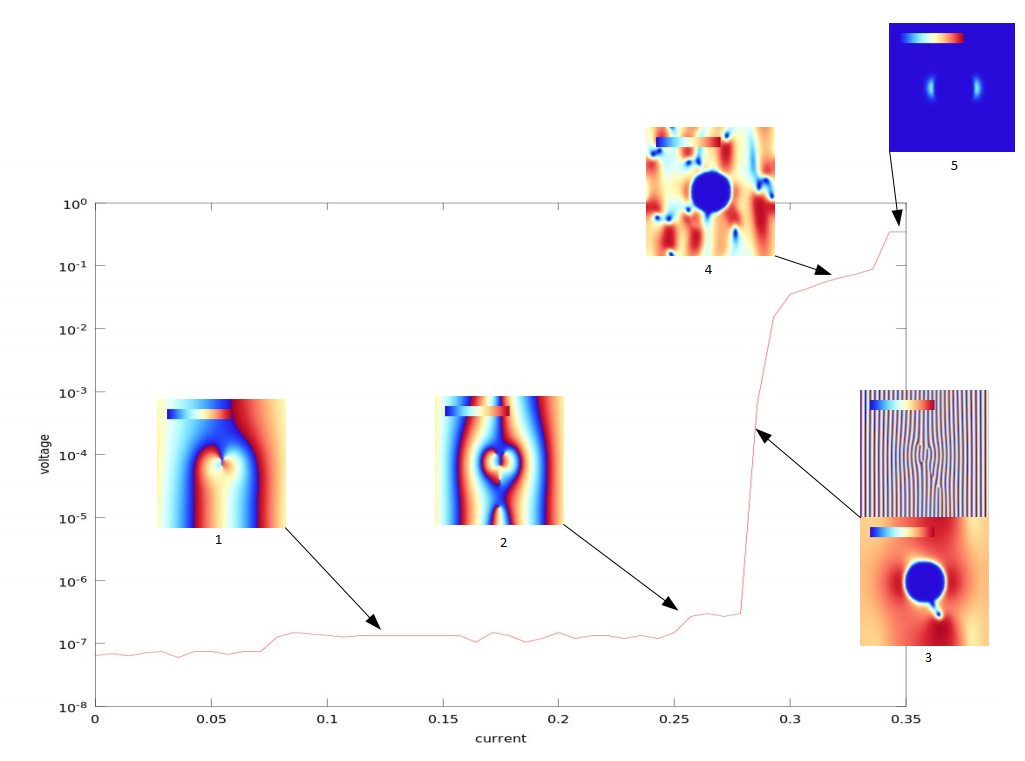
\includegraphics[scale=.50]{breakdownBreakdown.png}
\caption{This is a plot of the voltage (resistance) of the system as the current is slowly ramped up. At low currents, we just see the main vortex stuck to the Tc inclusion. As the current is increased, we eventually reach the depinning current and the vortices begin moving. This can be seen in the phase diagram as the phase has begun to wind up, indicating vortex movement. Sometime phenomena that can be observed, is that anti-vortex/vortex pairs are created in the inclusion and propagate in opposite directions. In region 3, the vortices clearly wind up the phase diagram and the resistance increases dramatically. Eventually in region 4, the system destabilizes and we begin to get vortex/anti-vortex pairs from the substrate. Finally, in region 5, we get full breakdown due to current and the system is no longer superconducting.}
\label{breakdown}
\end{center}
\end{figure}

